\chapter[Usefull and handy theorems in \texorpdfstring{\ensuremath{C^*}}{C*}-algebras]{Usefull and handy theorems in \texorpdfstring{\mathbf{C^*}}{C*}-algebras}

\section[\texorpdfstring{\ensuremath{C^*}}{C*}-algebras 101]{\texorpdfstring{\mathbf{C^*}}{C*}-algebras 101}



\begin{definicao}
\label{def: C* algebras}
\iftagged{BR}{
    Em uma álgebra $A$ (complexa), uma \tetxit{involução} é uma operação $a \longmapsto a^*$ que satisfaz: linearidade conjugada; ordem 2 e anti-comutatividade. Ou seja:
}{
    In a (complex) algebra $A$, it is called an \textit{involution} an operation $a \longmapsto a^*$ attending: conjugate-linearity,  order 2 and anti-commutativite. That is:
}
\begin{eqspaced*}{(a,b \in A, \lambda \in \C)}
    (a+\lambda b)^* = a^*+ \con \lambda b^*; \hspace{1cm} a^{**}=a; \hspace{1cm}(ab)^* = b^*a^*
\end{eqspaced*}
\iftagged{BR}{Se $(A,\|\come\|)$ for uma álgebra Banach e a involução satisfizer}{If $(A,\|\come\|)$ is a Banach algebra\footnote{Norm Cauchy-complete and submultiplicative $\|ab\|\leq \|a\|\cdot \|b\|$.} and the involution satisfies} $\|a^*a\|=\|a\|^2$ \iftagged{BR}{para todo $a$ (propriedade $C^*$), então $A$ é batizada de \textit{$C^*$-álgebra}.}{for all $a$ ($C^*$-property), then $A$ its said to be an \textit{$C^*$-algebra}. Setting $*$-morphisms to be the algebraic morphisms that respect involution\footnote{That is to say, linear maps $\phi : A \longto B$ such that $\phi(a^*)= \phi(a)^*$ for every $a\in A$.}, we construct the category of $C^*$-algebras $\Cstar \coloneqq \CstarOver{\C}$.}
\end{definicao}

\begin{exemplos} Some of the following examples are relatively bizarre for an initial view of the theory, but these represent important applications of $C^*$-algebras.
\begin{itroman}
    \item \iftagged{BR}{A carapuça naturalmente serve nos conjunto dos números complexos com a conjugação. Como $\C$ é completo, é uma $C^*$-álgebra.}{The complex conjugation in $\C$ naturally fits into the definition of an involution. Since $\C$ is complete, it is a $C^*$-algebra.}
    \item The square matrices algebra $\mathbb M_{n\times n}(\C)$ with $M\longmapsto {\con M}^t $ as the given involution is fated to also be an $C^*$-algebra.
    \item \label{item: C_b e C_0}For any $x \in \Top$ and $A \in \Cstar$, the algebras $C_b(x,A)$ and $\sub C0(x,A)$ of bounded and infinity-vanishing functions respectively, endowed with the point-wise involution\footnote{$f^* : x \longmapsto f(x)^*$ for any $f:x\longto A$.} also becomes $C^*$-algebras. 
    \item \textbf{Concrete \ensuremath{\boldsymbol{C^*}}-algebras}: Every $*$-closed subalgebra\footnote{A subalgebra $A$ for which $T\in A \Rightarrow T^* \in A$.} of bounded operators $T$ over a Hilbert space fits the above definition, since $\langle Tx,y\rangle = \langle x,T^*y\rangle$. In fact, the first $C^*$-algebras in town where precisely these, called the \textit{concrete} $C^*$-algebras. \cite{segal1947irreducible} introduced the term to describe preciselly these mathematical beings, to which he refers to as ``uniformly closed, self-adjoint algebra of bounded operators on a Hilbert space''. 
    
    %\item \textbf{\ensuremath{\boldsymbol{\sub C0(x)}}-algebras}
    
    \item \textbf{Irrational rotation algebra}: Let $\theta \in \R \backslash \Q$ be an irrational number. For $S^1 \coloneqq \{z\in \C \mid |z|=1\}$, consider $L^2(S^1)$ the Hilbert space of square-integral functions\footnote{$f:S^1 \longto \C$ whose $\int |f(z)|^2\de z < \infty$.} and the operators $U$ and $V$ given by:
    \begin{eqspaced*}{(z\in S^1)}
        Uf(z) \coloneqq z\cdot f(z) \e Vf(z) \coloneqq f(e^{2\pi i \theta} z)
    \end{eqspaced*}
    One should check that $VU = e^{2\pi i \theta} UV$. The $C^*$-algebra generated by $\{U,V\}$ is denoted by $A_\theta$. It is known that $A_{\theta}$ is a simple algebra (contains no bilateral ideals) and also that for $0<\theta_{1}<\theta_{2}<1 / 2$, the algebras $A_{\theta_{1}}$ and $A_{\theta_{2}}$ are not isomorphic (\cite{rieffel1981c}, Theorem 2). The proofs of these two facts are closely linked to the great advance of the theory of ${C}^{*}$-algebras in the last twenty-five years.
    
    \item \textbf{Toeplitz algebras and the Hardy Space}: Consider the \textit{shift} operator $T: H\longto H$ in separable Hilbert space $H$, given by $Te_n \coloneqq e_{n+1}$  where $(e_n)_{n\in \N}$ is an orthonormal basis. The \textit{Toeplitz algebra} is the smallest $C^*$-subalgebra $\mathscr T(H) \subset \mathscr B(H)$ containing $T$. 
    
    % https://lmbp.uca.fr/~yuncken/Teaching_docs/C-star-algebras.pdf
    Is a prototypical example of a Toeplitz algebra the \textit{Hardy space} $\mathscr H^2(S^1) \subset L^2(S^1)$ whose elements are precisely those $f\in L^2(S^1)$ in which all the negative Fourier coefficients are zero. 
    
    One of the most surprising observations about Toeplitz algebras is the fact that $\mathscr T(H)$ does not depend on $H$ nor on the orthonormal basis $(e_n)_n$ (up to isomorphism). 
%    \vspace{-0.65cm}
    \begin{quote}       \begin{invocacao}[\cite{douglas1998banach}, Theorem 7.23]
        Let $H$ be a Hilbert space and $\mathscr K(H) \subset \mathscr T(H)$ be the ideal of compact operators over $H$. There exists a $*$-isomorphism  
        \begin{equation*}
            \mfrac{\mathscr T(H)}{\mathscr K(H)} \longto C(S^1)
        \end{equation*}
        mapping the class of the shift operator into the identity $\sub{\Id}{C(S^1)}$.
    \end{invocacao}
    \end{quote}
    In fact, $\mathscr T(H)$ is the universal unital $C^*$-algebra generated by an isometry, providing a more categorical definition of an Toeplitz algebra: 
%    \vspace{-0.65cm}
    \begin{quote}
        \begin{invocacao}[Coburn]
            For any unital $A \in \Cstar^{\textit{\textbf{u}}}$ and any isometry $w \in A$, there is a unique unital $*$-morphism $\mathscr T(H) \longto A$ mapping the shift operator into $w$.
        \end{invocacao}
    \end{quote}
    To list one important aplication, \cite{cuntz1984k} provide a simple proof of Bott periodicity for $C^*$-algebras, in which only the functorial properties of $\sub K0$ and $\sub K1$ are required. The heart of the proof consists in the usage of the short exact sequence:
    $$0 \longto \mathscr K(\ell^2(\N))\longto \mathscr T(\ell^2(\N)) \longto C(S^1) \longto 0.$$
\end{itroman}
\end{exemplos}

\begin{definicao}[Invertible elements]
An element $a\in A$ in a unital ring, is said to be \textit{invertible} when there exists $b\in A$ such that $ab=ba=1$. The set of invertibles are denoted by $\GL(A)$.
\end{definicao}

\begin{proposicao}
\label{prop:invertiveis em A}
Let $A$ be a unital algebra and let $a,b,c \in A$.
\begin{itroman}
    \item If $a$ is invertible, then there is a unique $b$ such that $ab=ba=1$, and therefore, it can be denoted by $\inv a$.
    \item If $ab=ca=1$, then $b=c$ and hence $a$ is invertible. 
    \item If $ab=ba$, then $ab$ is invertible if and only if both
$a$ and $b$ are invertible.
    \item \label{prop:a*^-1 = (a^-1)*} If $A$ is an involution algebra, $a \in \GL(A) \Rightarrow \inv{(a^*)} = (\inv a)^*$.
\end{itroman}
\end{proposicao}
\begin{proof}$\left.\right.$
    \begin{itroman}
        \item Whenever $b$ and $b'$ are the interesting ones, $b(ab) = b(ab') = (ba)b' = b'$. 
        \item Notice that $c=c(ab) = (ca)b=b$.
        \item If $a$ and $b$ are invertible, therefore 
        \begin{equation*}
            ab(\inv a\inv b) = ba\inv a\inv b = 1 = \inv a\inv bba=(\inv a\inv b)ab.
        \end{equation*}
        Now, suppose that $ab$ is invertible and let $c \coloneqq \inv{(ab)}$. 
        \item Using the anti-commutativity of the involution,
        \begin{equation*}
            a^*(\inv a)^* = (\inv aa)^* = 1 = (a\inv a)^* = (\inv a)^*a^*,
        \end{equation*}
        that is to say, $\inv{(a^*)} = (\inv a)^*$. \qedhere
    \end{itroman}
    \end{proof}

Proposition \ref{prop:invertiveis em A} shows that $\GL(A)$ is a group under multiplication. 

\begin{definicao}[Spectrum]
For a unital Banach algebra $A$, the \textit{spectrum} of an element $a\in A$ is the set of scalar $\lambda$ such the elements $a-\lambda \coloneqq a - \lambda1$ aren't invertible, i.e.,
\begin{equation*}
    \Spec(a) \coloneqq \{\lambda \in \C \mid a-\lambda \notin \GL(A)\}.
\end{equation*}
For non-unital Banach algebras, since $A$ can be isometrically embeded into a unital algebra $A^u$, $\Spec(a)$ stand for the spectrum over its identification. 
\end{definicao}

\begin{exemplos}$\left.\right.$
\begin{itroman}
\item Let $x$ be a compact Hausdorff topological space, we'll show that $\Spec(f) = \Im f$ for every continuous function $f\in C(x)$. Given $\lambda\in \Spec(f)$, notice that $f - \lambda \textit{1}$ is non-invertible if and only if, there exists $x\in x$ such that  $(f- \lambda \textit{1})(x) = 0$, which means $f(x) = \lambda$.

\item Whenever $T\in \mathbb M_{n}(\C)$, $\Spec T$ stands for the set of eigenvalues of $T$, due to the fact that those values $\lambda$ are the ones that $\det(T-\lambda \Id_n)=0$; precisely the operators which $T-\lambda \Id_n$ aren't invertible.

\item Let $A$ be a unital $C^*$-algebra and $a\in A$. Let $\lambda$ be a complex number. By proposition \ref{prop:invertiveis em A}\ref{prop:a*^-1 = (a^-1)*} it is safe to say that $a-\con \lambda = (a^*-\lambda)^*$ isn't invertible if and only if $a^*-\lambda$ isn't as well. Therefore, $\Spec(a^*) = \con{\Spec(a)}$.
\end{itroman}
\end{exemplos}

\begin{lema}
\label{lema: Spec(ab)-0 = Spec(ba)-0}
For elements $a, b$ in a $C^*$-algebra $A$, $\Spec(a b) \backslash\{0\}=\Spec(b a) \backslash\{0\}$.
\end{lema}
\begin{proof}
Assume that $A$ is unital. It suffices to prove that $1-a b \in \GL(A)$ implies $1-b a \in \GL(A)$
Let $u\coloneqq (1-a b)^{-1}$. Then
\begin{equation*}
    \begin{array}{rcl}
(1+b u a)(1-b a) &=& 1-b a+b u a-b u a b a \\
&=& 1-b(1-u+u a b) a \\
&=& 1-b(1-u(1-a b)) a =1
\end{array}
\end{equation*}
Similarly $(1-b a)(1+b u a)=1$. Hence $1-b a \in \GL(A)$.
\end{proof}


\begin{lema}
\label{lema:lambda1-a invertivel para ||a||<lambda}
\iftagged{BR}{Em uma álgebra de Banach unitária $A$, se $\lambda \in \mathbb{C}$, os elementos da forma $\lambda-a$ com $a \in A$, são invertíveis se $\|a\|<|\lambda|$. Além disso, qualquer morfismo de álgebras da forma $\phi: A \longrightarrow \mathbb{C}$ é contínuo e $\|\phi\| \leqslant 1$.
}{In a unitary Banach algebra $A$, if $\lambda \in \mathbb{C}$, elements of the form $\lambda-a$ with $a \in A$, are invertible if $\|a\|<|\lambda|$. Furthermore, any algebraic morphism of the form $\phi: A \longrightarrow \mathbb{C}$ is continuous and $\|\phi\| \leqslant 1$.}
\end{lema}
\begin{proof}
   Consider the sequence of partial sums of the form $1+a / \lambda+a^{2} / \lambda^{2}+\cdots+a^{n} / \lambda^{n}$, and notice that they forms a Cauchy sequence, so it converges to a element $b$, given that $\|a / \lambda\|<1$. Notice that
$$
\lambda\Big(1-\frac{a}{\lambda}\Big) \underbrace{\lim _{n \rightarrow \infty} \sum_{j=0}^{n}\Big(\frac{a }{\lambda}\Big)^{j}}_{b}=\lim _{n \rightarrow \infty} \lambda\Big(1-\frac{a^{n+1}}{\lambda^{n+1}}\Big)=\lambda
$$
So $\left(\lambda-a\right)^{-1}=b$. Without loss of generality, we can assume that $\phi$ is non-null and $\phi\left(1\right)=1$. As we have seen,
$$
\left(\lambda-a\right) b=1 \hspace{0.25cm}\Rightarrow\hspace{0.25cm}(\lambda-\phi(a)) \phi(b)=1,
$$
meaning $\phi(a) \neq \lambda$. Since this holds for all $\lambda$ such that $|\lambda|>\|a\|$, it follows that $|\phi(a)| \leqslant$ $\|a\|$, which proves our claim that $\|\phi\|\leqslant 1$.
\end{proof}

\begin{proposicao}
\label{prop: GL(A) eh aberto}
The group $\GL(A)$ of invertible elements in a unitary Banach algebra $A$ constitute an open set.
\end{proposicao}
\begin{proof}
Let $x$ be an invertible. Given $y$ such that $\|x-y\| < \inv{\|\inv x\|}$, let's see that $y$ will be an invertible as well. From the asssumption and submultiplicativity of the norm, its easy to see that
\begin{equation*}
    \|1-\inv xy\|=\|\inv x(x-y)\| \leq \|\inv x\|\|x-y\| <\|\inv x\| \inv{\|\inv x\|} = 1,
\end{equation*}
hence $1-(1-\inv xy) = \inv xy$ is invertible by \ref{lema:lambda1-a invertivel para ||a||<lambda}. But since $\GL(A)$ is a group, $y$ must also be invertible, i.e., the open ball around $x$ of radious $\inv{\|\inv x\|}$ is fully contained in $\GL(A)$, so it is open.
\end{proof}

\begin{proposicao}
\label{prop: inversao eh continua}
Over a unitary Banach algebra $A$, the invertion map $a\longmapsto \inv a$ is a continuous function. 
\end{proposicao}
\begin{proof}
Choose $x,y\in \GL(A)$ such that $\|x-y\| < \inv{\|\inv x\|}$. As showed in the proof of \ref{prop: GL(A) eh aberto}, $\|1-\inv xy\| < 1$ and therefore,
\begin{equation}
\label{eq: inv y dentro de GL(A)}
\begin{array}{rl}
         & \inv yx = \inv{1-(1-\inv xy)} =  \displaystyle\sum\limits_{n=0}^\infty (1-\inv xy)^n \\
    \Rightarrow & \hphantom{x}\inv y = \displaystyle\sum\limits_{n=0}^\infty (1-\inv xy)^n\inv x
\end{array}
\end{equation}
If we want to estimate how close $x$ and $y$ need to be in order that $\|\inv y-\inv x\|$ can be arbitrally small, (\ref{eq: inv y dentro de GL(A)}) might help to found an upper bound:
\begin{equation*}
    \|\inv y - \inv x\| = \Big\| \displaystyle\sum\limits_{n=1}^\infty (1-\inv xy)^n\inv x \Big\| \leqslant \|\inv x\| \displaystyle\sum\limits_{n=1}^\infty \|1-\inv xy\|^n = \|\inv x\| \cdot \dfrac{\|1-\inv xy\|}{1-\|1-\inv xy\|}
\end{equation*}
For a given $\ep>0$, since $t \longmapsto t/(1-t)$ is a increasing continuous function for $t<1$, there allways exists $\delta_{x,\ep}>0$ right for the job:
$$t < \delta_{x,\ep} \coloneqq \dfrac{\frac\ep{\|\inv x\|}}{\frac\ep{\|\inv x\|} + 1}  \hspace{0.2cm}\Rightarrow \hspace{0.2cm}\dfrac{t}{1-t} < \frac\ep{\|\inv x\|}, $$
so whenever $\|x-y\|<\delta_{x,\ep}$, $\|\inv y - \inv x\|<\ep$.
\end{proof}

\begin{proposicao}
\label{prop: R_a eh holomorfa}
The \textit{resolvent function} (\ref{eq: resolvent function}) is holomorphic for each and every unital Banach algebra $A$.
\begin{eqspaced}{(a\in A)}
    \label{eq: resolvent function}
    \function{{R_a}{\C\backslash \Spec(a)}{A}{\lambda}{\inv{(\lambda-a)} = \displaystyle \sum\limits_{n=0}^\infty \Big(\frac a\lambda\Big)^n}}
\end{eqspaced}
\end{proposicao}
\begin{proof}
Let $z,w \in \C \backslash\Spec(a)$. Let $\alpha \coloneqq z-a$ and $\beta \coloneqq w-a$. Notice that
\begin{eqnarray*}
    R_a(z) - R_a(w) &=& \inv\alpha - \inv\beta \\ &=&\inv{\alpha}\big(1 - \alpha \inv\beta\big)
    \\ &=&\inv{\alpha}\big(\beta - \alpha \big)\inv\beta \\
    &=& R_a(z)(w-z)R_a(w)
\end{eqnarray*}
Therefore:
\begin{eqspaced*}{(z\in \C\backslash \Spec(a))}
    \hspace{-0.5cm}\lim_{w\to z} \dfrac{R_a(z)-R_a(w)}{z-w} = 
    \lim_{w\to z} -R_a(z)R_a(w) = -R_a(z)^2 
\end{eqspaced*}
So the limit exists, $\partial R_a = -R_a^2$ and it is analytic over the domain.
\end{proof}

%\begin{invocacao}[Liouville]
%    \label{invocacao: liouville}
%    Every non-constant holomorphic \textit{entire}\footnote{I.e., that is analytic in the whole complex plane.} function $f$ in the complex plane has unbounded image. Conversely, if there exists $M>0$ such that $|f(z)| \leqslant M$ for each complex $z$, then $f$ necessarily must be constant. A simple proof over harmonic functions can be found in \cite{nelson1961proof}.
%\end{invocacao}

\begin{teorema}
\label{teo:spec eh compacto}
The spectrum of any element $a$ in a Banach algebra is a compact non-empty set, and satisfies:
\begin{equation*}
    \Spec(a) \subset \{\lambda \in \C \mid |\lambda| \leqslant \|a\|\}.
\end{equation*}
\end{teorema}
\begin{proof}
Since life is really good and Heine-Borel's theorem holds for complex numbers, we need only to show that $\Spec(a)$ is closed and bounded.
\begin{itroman}
\item \textbf{$\boldsymbol{\Spec(a)}$ is a closed set}. Since $a$ is fixed element, notice the projection ${a+\lambda}\longmapsto {\lambda}$ is a continuous function by \ref{lema:lambda1-a invertivel para ||a||<lambda} and so is their inverse $\lambda \longmapsto a-\lambda$. Since $\Spec(a)$ is the set-theoretic complement of the pre-image of $\GL(A)$ (an open set - \ref{prop: GL(A) eh aberto}) by a continuous function, it must be closed.

\item \label{teo item:spec eh limitado}\textbf{$\boldsymbol{\Spec(a)}$ is bounded}. From \ref{lema:lambda1-a invertivel para ||a||<lambda}, spectral elements of the form $\lambda-a$ must necessarily obey $|\lambda| \leq \|a\|$, i.e., $\Spec(a) \subset \{\lambda \in \C \mid |\lambda|\leqslant\|a\|\}$.
\end{itroman}
Therefore, $\Spec(a)$ is compact set. In order to give a little bit of flavor, we present the proof of \cite{singh2006spectrum} the non-emptiness of the spectrum, with a clever tricky about derivation under the integral sign.
\begin{enumerate}[label=\ensuremath{(\roman*)}]
    \setcounter{enumi}{2}
\item \label{teo item:spec eh n vazio}\textbf{$\boldsymbol{\Spec(a)}$ is non-empty}. Suppose $a\neq 0$, since otherwise the result follows immediately. Assume that $\Spec(a)$ is empty, so that $R_a$ exists in all complex plane. In particular, $a \in \GL(A)$. For any bounded linear functional $f: A\longto \C$, the function 
\begin{equation*}
    \function{{\sub gf}{\R^2}{\C}{(r,\theta)}{f(R_a(re^{i\theta}))}}
\end{equation*}
is continuously differentiable with respect to both $r$ and $\theta$:
\begin{equation}
\label{eq: spec eh n vazio: derivadas de g}
    \sub\partial\theta {\sub gf}(r, \theta)=f\big(-R_a(r e^{i \theta})^{2}\big) i r e^{i \theta} \e
\partial_r{\sub gf}(r, \theta)=f\big(-R_a(r e^{i \theta})^{2}\big) e^{i \theta}.
\end{equation}
Hence $\sub\partial\theta {\sub gf} = ir\partial_rg$. Now let $F(r)\coloneqq \int_{0}^{2 \pi} {\sub gf}(r, \theta)\,\de\theta$. By differentiating under the integral sign\footnote{Such a differentiation is possible, since $g$ is clearly a $C^{1}$-function by (\ref{eq: spec eh n vazio: derivadas de g}).} and using $\partial_r{\sub gf}$, we obtain
\[
\begin{aligned}
F^{\prime}(r)&=\int\limits_{0}^{2 \pi} \partial_r{\sub gf}(r, \theta)\,\de\theta=\int\limits_{0}^{2 \pi} f\big(-R_a(r e^{i \theta})^2\big) e^{i \theta} \,\de\theta\\
\Rightarrow \hspace{0.5cm} ir F^{\prime}(r) &=\int\limits_{0}^{2 \pi} f\big(-R_a(r e^{i \theta})^{2}\big) i r e^{i \theta} \,\de\theta=\int\limits_{0}^{2 \pi} \sub\partial\theta {\sub gf}(r, \theta) \,\de \theta \\
&=f(R_a(r e^{i 2\pi}))-f(R_a(r e^{i 0}))=0\\
\Rightarrow \hspace{0.5cm} F(r) &=F(0)=2 \pi f(a^{-1})
\end{aligned}
\]
We now choose $f$ so that $f\left(a^{-1}\right) \neq 0$. Let $h : \operatorname{Span}(\inv a) \longto \C$, $h(z\inv a) = z\|\inv a\|$. Since $\|\come\|$ is a positive sublinear functional, we are able to conjure: 
\begin{quote}
%\vspace{-0.75cm}
    \begin{invocacao}[Complex Hahn-Banach]
        Let $X$ be a $\mathbb K$-vector space with $\mathbb K \in \{\R,\C\}$ and $p$ a positive sublinear functional\footnote{I.e., for all vectors $x,y$ and scalar $\alpha$, $p(x)\geq 0$, $p(x+y)\leq p(x)+p(y)$ and $p(\alpha x) \leq |\alpha|p(x)$.}. If $Y \subset X$ is a subspace and $h : Y \longto \mathbb K$ a linear functional dominated by $p$ (i.e., $|h(y)| \leq p(y)$ for $y\in Y$), the there exists a \textit{Hahn-Banach extension} $f: X \longto \mathbb K$ such that $f$ is also dominated by $p$. 
    \end{invocacao}
\end{quote}
Therefore, choose a Hahn-Banach extension $f$ of $h$ such that $f(\inv a) = \|\inv a\| \neq 0$. Since
$$
f\big(R_a(r e^{i \theta})\big)=f\big(\inv{(re^{i\theta}1-a)}\big) = r^{-1} e^{-i \theta} f\big((1-a r^{-1} e^{-i \theta})^{-1}\big)
$$
it follows that $\big|f\big(R_a(r e^{i \theta})\big)\big|$ can be made as small as we like, independently of $\theta$, by choosing $r$ sufficiently large, by the continuity of the invertion map $ x \longmapsto x^{-1}$ (\ref{prop: inversao eh continua}). We fix $r$ such that $\big|f\big(R_a(r e^{i \theta})\big)\big|<\big|f(a^{-1})\big| / 2$. For this $r$ we have
$$
2 \pi|f(a^{-1})|=|F(r)| \leq \int\limits_{0}^{2 \pi}\big|f\big(a(r e^{i \theta})\big)\big|\,\de\theta \leq \pi\big|f(a^{-1})\big|
$$
which is not possible. Therefore, $\Spec(a)$ must in fact be non-empty.
%Supose otherwise, $\C \backslash \Spec(a) = \C$. In that case, proposition \ref{prop: R_a eh holomorfa} tell'us that $R_a$ is an \textit{entire} function, analytic and bounded by \ref{teo item:spec eh limitado}. %Liouville's theorem \ref{invocacao: liouville} would garantee us that $R_a$ must be constant, which is ridiculous!
\end{enumerate}
\end{proof}

Typically, in order to prove \ref{teo:spec eh compacto}\ref{teo item:spec eh n vazio}, one would argue that if otherwise, $R_a$ would be \textit{entire} function and conclude that it must constant by Liouville's theorem. The advantage of the argument presented, as showed in \cite{singh2006spectrum}, is a more elementary proof, and both the fundamental theorem of Algebra and Liouville's theorem as corollary.

\begin{corolario}[Fundamental Theorem of Algebra]
\label{teo: fund. teo. algebra}
If $p\in \C[z]$, there exists a complex root $w\in \C$ such that $p(w)=0$.
\end{corolario}
\begin{proof}
In the algebra of complex square matrices $\mathbb M_n(\C)$, set $T$ as the operator in which $p$ is the characteristic polynomial. If $p(z) = z^n + \alpha_{n-1}z^{n-1} + \cdots + \sub\alpha1z + \sub\alpha0$, one may let
$$
T \coloneqq 
\left[\begin{array}{ccccc}
0 & 0 & \cdots & 0 & -\sub\alpha{0} \\
1 & 0 & \cdots & 0 & -\sub\alpha{1} \\
0 & 1 & \cdots & 0 & -\sub\alpha{2} \\
\vdots & \vdots & \ddots & \vdots & \vdots \\
0 & 0 & \cdots & 1 & -\alpha_{n-1}
\end{array}\right]
$$
By \ref{teo:spec eh compacto}\ref{teo item:spec eh n vazio}, there exists an eigenvalue $w \in \Spec T$ thus $p(w)=0$.
\end{proof}

\begin{corolario}[Liouville's Theorem]
Let $A\in \BAlg^{\textit{\textbf{u}}}$ be a unitary Banach algebra. If $f:\C \longto A$ is a bounded function which is holomorphic everywhere (i.e., \textit{entire}), then it must be constant.
\end{corolario}
\begin{proof}
Let $f$ be a bounded entire function. Fix an arbitrary $w\in \mathbb{C}$. Define $g$ on $\mathbb{C}$ as follows:
$$
g(z)\coloneqq \begin{cases}(f(z+w)-f(w)) / z & \text { if } z \neq 0. \\ f^{\prime}(w) & \text { if } z=0.
\end{cases}
$$
Then $g$ is certainly continuous in $\mathbb{C}$ and analytic in $\mathbb{C}_{\neq 0}$. Define $F(r)=\int_{0}^{2 \pi} g(r e^{i \theta})\,\de\theta
$. By the same idea used in the argument of \ref{teo:spec eh compacto}\ref{teo item:spec eh n vazio}, $F$ must be constant. However, from the boundedness of $f$ it follows that $g$ tends to 0 uniformly in $\theta$ as $r$ tends to infinity, so $F$ tends to 0. Therefore, $F(r)=F(0)=0=2 \pi f^{\prime}(w)$. As $w$ was an arbitrary point of $\mathbb{C}$, we conclude that $f^{\prime}$ is identically zero, therefore $f$ is constant.
\end{proof}

\begin{teorema}[Spectral Mapping Theorem]
\label{teo: spectral mapping}
Given an unital Banach algebra $A$ and $a\in A$, the following holds for each complex-polynomial:
\begin{eqspaced*}{(p \in \C[x])}
    \Spec(p(a)) = \{p(\lambda) \mid \lambda \in \Spec(a)\} = p(\Spec(a)).
\end{eqspaced*}
\end{teorema}
\begin{proof}
Fix $p \in \C[x]$ and by the Fundamental Theorem of Algebra \ref{teo: fund. teo. algebra}, for each $\lambda \in \C$, it is possible to decompose $\lambda-p(z)$ into linear factors. By the Cayley-Hamilton theorem, it is safe to say that there is $\sub\lambda, \ldots, \lambda_n, \alpha\in \C$ such: 
\begin{eqspaced*}{(a\in A)}
\lambda-p(a) = \alpha \prod_{i=1}^n(\lambda_i1-a).
\end{eqspaced*}
If $\lambda_i \notin \Spec(a)$ for each index $i$, every factor $\lambda_i1-a$ is invertible, hence $\lambda - p(a)$ are as well. In order to $\lambda \in \Spec(p(a))$, there must exist a root $\lambda_j$ such that $\lambda_j \in \Spec(a)$. In that case, $\lambda = p(\lambda_j) \in p(\Spec(a))$, and we shall conclude that $\Spec(p(a)) \subset p(\Spec(a))$.  

To prove the other inclusion, let $\lambda \in p(\Spec(a))$, meaning that there is $\eta \in \C$ such that $\eta1-a$ is non-invertible and $p(\eta)=\lambda$. But because decomposition is unique, there must be $j$ such that $\eta = \lambda_j$ and by the same argument, one concludes that $\Spec(p(a)) \supset p(\Spec(a))$, obtaining the equallity.
\end{proof}

\begin{observacao}
In quantum mechanics, physical observables are represented mathematically by linear operators on Hilbert spaces. One remarkable corollary of the non-emptiness of the spectrum imply that, it is not possible to describe the position and momentum operators as elements of a Banach algebra. 
\begin{quote}
    \textbf{Proposition}. The \textit{Weyl algebra} $\mathbb{C}\left[x, \partial_{x}\right] \simeq \mfrac{\mathbb{C}[x, y]}{(y x-x y-1)}$ does not embed into a Banach algebra.
    \vspace{-0.4cm}
    \begin{proof}
    Suppose to the contrary that $x, y$ are elements of a Banach algebra satisfying $y x-x y=1$. From the spectral mapping theorem \ref{teo: spectral mapping},
    \begin{center}
        $\Spec(y x)=\Spec(x y+1)=\Spec(x y)+1.$
    \end{center}
    But we know that $\Spec(y x)=\Spec(x y)$, so the spectrum of the product $xy$ must be invariant under addition by 1. By non-emptyness, it must contain arbitrarily large elements, and this contradicts compactness.
    \end{proof}
\end{quote}
Hence, it is necessary to look at the unitary groups of strongly continuous functions that the position and momentum operators generate, through the Stone-von Neumann theorem, stating that, the canonical commutation relations on two generators (canonical coordinate $q$ and canonical momentum $p$) in the form $[q,p]=i\hbar$ may be represented as unbounded operators on the Hilbert space of square integrable functions $L^2(\R)$ on the real line by defining them on the dense subspace of smooth functions $\psi:\R\longto \C$ as
\begin{equation*}
    (q\psi)(x)\coloneqq x\psi(x) \e (p\psi)(x)\coloneqq i\hbar \partial_x\psi(x),
\end{equation*}
where on the right we have the derivative along the canonical coordinate function on real numbers axis.
\end{observacao}

\begin{corolario}[Complex Gelfand-Mazur]
\label{teo: Gelfand Mazur}
Any complex unital Banach division algebra $A$ (every non-zero element is invertible) is isometrically isomorphic to $\C$.
\end{corolario}
\begin{proof}
Let $a$ be a non-zero element, i.e., invertible. Since $\Spec(a)$ is non-empty \ref{teo:spec eh compacto}\ref{teo item:spec eh n vazio}, there must exist $\lambda_a$ such that $a-\lambda_a1$ isn't invertible. The only non-invertible elemen't in $A$ is the zero element, which means that $a = \lambda_a1$.
\end{proof}


\begin{teorema}[Beurling-Gelfand formula]
\label{teo: raio espectral}
The \textit{spectral radius} $r$ of an element $a\in A$ can be directly calculated by the following formula:
\begin{equation*}
    r(a) \coloneqq \sup |\Spec(a)| = \lim_{n\to \infty} \sqrt[n]{\|a^n\|}
\end{equation*}
for \textit{any Banach norm} $\|\,\cdot\,\|$.
\end{teorema}
\begin{proof}
By the Spectral Mapping theorem \ref{teo: spectral mapping} and the continuity of the inversion map \ref{prop: inversao eh continua}\ref{teo item:spec eh limitado}, is easy to estabilish that $r(a)^n = r(a^n) \leqslant \|a^n\| $ for any given natural $n$, hence $r(a) \leqslant \inf \|a^n\|^{1/n}$. Notice that if $|\lambda| > r(a)$, then $\lambda-a$ is invertible by \ref{lema:lambda1-a invertivel para ||a||<lambda}. For any bounded linear $\phi : A \longto \C$, the operator
\begin{eqspaced*}{(|\lambda|\geq r(a))}
    (\phi \circ R_a)\lambda = \phi(\inv{(\lambda - a)}) = \sum_{n=0}^\infty \dfrac1{\lambda^n}\phi(a^n)
\end{eqspaced*}
is analytic, and hence, converges absolutely. That can only happend if the general term of the series $\phi(a^n/\lambda^n)$ converges to 0 for any bounded linear $\phi$. Since every weakly convergent sequence is bounded (\ref{prop: convergia fraca eh limitada}), for each $\lambda$, there is $M_\lambda > 0$ such that $\|a^n\| \leqslant M_\lambda\, |\lambda^n|$. Therefore,
\begin{equation*}
    \underset{n\to \infty}{\operatorname{limsup}}\sqrt[n]{\|a^n\|} \leqslant 
    \underset{n\to \infty}{\operatorname{limsup}}\sqrt[n]{M_\lambda} |\lambda| = |\lambda|
\end{equation*}
Since this holds for every $|\lambda|>r(a)$ we have
$$
r(a) \leq \inf_{n\in\N} \sqrt[n]{\|a^n\|} \leq \underset{n \rightarrow \infty}{\operatorname{liminf}}\sqrt[n]{\|a^n\|} \leq \underset{n \rightarrow \infty}{\operatorname{limsup}}\sqrt[n]{\|a^n\|} \leq r(a),
$$
which finishes the proof.\end{proof}

\begin{exemplo}
In \ref{prop: inversao eh continua}\ref{teo item:spec eh limitado}, $\sup |\Spec(a)| \leqslant \|a\|$, but this inequallity can be strict: Over $\mathbb M_{2\times 2}(\C)$, notice that 
\begin{eqspaced*}{(t>0)}
    \sup \Big|\Spec \begin{pmatrix}
    0 & 1/t \\
    t & 0
    \end{pmatrix}\Big| = \sup |\{1,-1\}| = 1
\end{eqspaced*}
but $\left\|\begin{smallmatrix}
    0 & 1/t \\
    t & 0
    \end{smallmatrix} \right\| = t^2+ 1/t^2$.
\end{exemplo}

\begin{lema}
\label{lema: a*=a --> Spec a real}
Let $a\in A$ be an element of a $C^*$-algebra. If $a\in A$ is a self-adjoint, then $\Spec(a) \subset \R$.
\end{lema}
\begin{proof}
Let $\lambda \in \operatorname{Spec} (a)$. For each integer $n$, let $b_{n}\coloneqq a+(i n \Im \lambda-\operatorname{Re}\lambda)$. Considering the rational function $f$ given by $f(z)=z-\operatorname{Re}\lambda+i n \Im y$ we conclude that $f(\lambda) \in \operatorname{Spec} f(a)$ from the Spectral Mapping theorem \ref{teo: spectral mapping}. Hence, $i(n+1) \Im \lambda \in \operatorname{Spec} (b_{n})$.

From \ref{lema:lambda1-a invertivel para ||a||<lambda}, one obtains that $|i(n+1) \Im \lambda| \leqslant\left\|b_{n}\right\|$. Therefore
$$
\begin{array}{rcl}
(n^{2}+2 n+1) (\Im \lambda)^{2} &= &|i(n+1) \Im \lambda|^{2} \\
& \leqslant &\left\|b_{n}\right\|^{2} \\
&= &\left\|b_{n}^{*} b_{n}\right\| \\
&\overset{a^*=a}=&\|(a-\operatorname{Re}\lambda-i n \Im \lambda)(a-\operatorname{Re}\lambda+i n \Im \lambda)\| \\
&=& \|(a-\operatorname{Re}\lambda)^{2}+n^{2} (\Im \lambda)^{2}\| \leqslant\|a-\operatorname{Re}\lambda\|^{2}+n^2(\Im \lambda)^{2}
\end{array}
$$
which implies that $(2 n+1) (\operatorname{Im}\lambda)^{2} \leqslant\|a-\operatorname{Re}\lambda\|^{2}$. Since $n$ is arbitrary, it follows that $(\Im \lambda)^2$ is arbitrarily small, i.e., $\Im \lambda=0$, hence $\Spec(a) \subset \R$.
\end{proof}


\begin{lema}
If $a \in A$ is a self-adjoint element of a unitary $C^{*}$-algebra, then $r(a)=\|a\|$.
\end{lema}\begin{proof}
We have $\left\|a^{2}\right\|=\left\|a^{*} a\right\|=\|a\|^{2}$. We appeal to induction: Suppose $n$ is such that ${\|a^{2^{n}}\|}^{2^{-n}}=\|a\| $. Therefore:
$$
\left\|a^{2^{n+1}}\right\|^{2^{-n-1}}=\sqrt{\left\|\left(a^{2^{n}} \right)^{2}\right\|^{2^{-n}}}=\sqrt{\| a^{2^{n}} \|^{2^{-n}}} \stackrel{\text { I.H. }}{=} \sqrt{\|a\|^{2}}=\|a\|.
$$
By induction, the above assumption is valid for all natural $n$. Therefore, the sequence $\big(\left\|a^{n}\right\|^{1 / n}\big)_{n \in \mathbb{N}}$, which converges to $r(a)$ by \ref{teo: raio espectral}, has a constant subsequence equal to $\|a\|$. Then $r(a)=\|a\|$.
\end{proof}

\section{Gelfand-Naimark representation theorem}
To explore \ref{item: C_b e C_0}, both bounded and infinity-vanishing functions can be seeing as a contra-variant functor from topological spaces to abelian $C^*$-algebras. We will focus on the infinity-vanishing ones:  
\begin{equation*}
    \contfunctor{{\sub C0}{\Top}{\CstarCom}{X}{\sub C0(X)}{Y}{\sub C0(Y)}{f}{\,}{\phi}{\phi \circ f}}
\end{equation*}

\begin{definicao}[Gelfand transformation]
For a given $A\in \BAlg$, the \textit{character space} of $A$ is the set of non-zero morphisms ${{\GGamma}{A}} \coloneqq \Hom_{\BAlg}(A,\C)_{\neq 0}$. The \textit{Gelfand transformation} is the evaluation functional $\kappa \coloneqq \ev_{(\,\cdot\,)}$ given by:
\begin{equation}
\label{eq: transformada de gelfand}
    \function{{\kappa}{A}{\sub C0({{\GGamma}{A}})}{a}{(\phi \overset{\ev_a}\mapsto \phi(a))}}
\end{equation}
\end{definicao}

Later, we will endow a topological flavor onto $\GGamma{A}$. Before, we gave a look into a alternative definition of the character space.

\begin{proposicao}
If $A$ is a unitary commutative Banach algebra, let $\mathscr I_{m}(A)$ be the set of maximal ideals\footnote{We say that $I \subset A$ is an ideal if $I$ is closed by $A$-linear combinations, i.e., given $x, y \in I$ and $a, b \in A$, then $a x +b y \in A$. We denote $I \triangleleft A$. We say that $I \triangleleft_{m} A$ is a maximal ideal if it is not trivial (like $\{0\}$ or $A$ ) and if any other ideal $J \triangleleft A$ such that $I \subset J \subset A$ collapses with either $I$ or $A$.} of $A$. So the function $\ker(\come): \GGamma{A} \longrightarrow \mathscr I_{m}(A)$ is a bijection. Since in algebraic lands $\mathscr I_{m}(A)$ is often called \textit{spectrum of $A$}, the character space may also be called the \textit{spectrum}.  
\begin{proof}
Of course $\operatorname{ker}(\,\cdot\,)$ is well defined, i.e. $\operatorname{ker} \phi$ is always a maximal ideal of $A$ for any character $\phi$. That's because $\phi$ is necessarily surjective ($\phi\left(z 1_{A}\right)=z \phi\left(1_{A}\right)=z$ for any $z \in \mathbb{C}$) and by the First Isomorphism Theorem, $A / \operatorname{ker} \phi \simeq \mathbb{C}$ is a field and therefore, $\operatorname{ker} \phi$ is maximal (since $A$ is a commutative ring).

In order to $\ker(\,\cdot\,)$ be a bijection, we verify:
\begin{itroman}
    \item \textbf{$\boldsymbol{\operatorname{ker}(\,\cdot\,)}$ is an injection}: Let $\phi, \psi \in \widehat{A}$ characters such that $\operatorname{ker} \phi= \ker \psi$. Notice that
    \begin{eqspaced*}{(a\in A)}
    \phi(a) 1_{A}-a \in \operatorname{ker} \phi=\operatorname{ker} \psi
    \end{eqspaced*}
That is, $\psi\left(\phi(a)1-a\right)=0$ from which it follows that $\phi=\psi$.
\item \textbf{$\boldsymbol{\operatorname{ker}(\,\cdot\,)}$ is a surjection}: Let $I \triangleleft_{m} A$ be a maximal ideal and consider the projection $\sub\pi{I}: x \longmapsto x+I$. So $\ker \sub\pi{I}=I$. It remains to verify that $\sub\pi{I}$ is a character but this will follow from the fact that $A / I$ is a Banach algebra where all its elements are invertible.

Since $I$ is maximal it follows that $A / I$ is a field and in particular an algebra. Using the Gelfand-Mazur theorem \ref{teo: Gelfand Mazur}, all non-zero elements of $A / I$ are all invertible and therefore we guarantee that $A / I \simeq \mathbb{C}$. 
\end{itroman}
This concludes the proof.
\end{proof}
\end{proposicao}

\begin{lema}
\label{lema: specm A eh localmente compacto}
Endowed with the weak* topology, ${{\GGamma}{A}}$ is a locally compact Hausdorff topological space. Whenever $A$ is unitary, then ${{\GGamma}{A}}$ is compact.
\begin{proof}
The weak* topology on ${{\GGamma}{A}} \subset \mathscr B(A,\C)$ is induced by the \textit{separant}\footnote{I.e., given an arbitrary $a$, there exists $\phi\in \GGamma A$ such that $|\phi(a)|\neq 0$} familly of seminorms $({p_a})_{a\in A}$ given by $p_a : \phi \longmapsto |\ev_a(\phi)|=|\phi(a)|$, in the sense that it is the smallest topological space such that each $p_a$ be continuous. Therefore, ${{\GGamma}{A}}$ is a Hausdorff topological vector space. 

Let $S \coloneqq \Hom_{\Cstar}(A,\C)$ for convention. We afirm that:
\begin{itroman}
    \item \label{item: S é fechado}\textbf{$\boldsymbol{S}$ is a closed subspace of the unity ball over $\boldsymbol{\mathscr B(A,\C)}$}: Let $B$ be the unit ball on the dual space and choose $\phi\in B$. For any net $(\sub\phi\lambda)_\lambda \subset S$ whoose $\lim_\lambda \sub\phi\lambda = \phi$, one have
    \begin{eqspaced*}{(a,b\in A)}
    \begin{array}{rcl}
         \phi(ab) &=& \displaystyle \lim_\lambda \sub\phi\lambda(ab) \\ &\overset{\sub\phi\lambda \in S}=& \displaystyle \lim_\lambda \sub\phi\lambda(a)\sub\phi\lambda(b) \\ &=& \displaystyle \lim_\lambda \sub\phi\lambda(a)\, \lim_\lambda \sub\phi\lambda(b) = \phi(a) \phi(b)
    \end{array}
    \end{eqspaced*}
    i.e., $\phi \in S$, hence it is a closed subspace.
    \item \label{item: A unital ==> 0 é pto isolado}\textbf{Whenever $\boldsymbol A$ is unitary, $\boldsymbol{ \textit{0}: x\longmapsto 0}$ is a isolated point of $\boldsymbol{S}$}: For any net $(\sub\phi\lambda)_\lambda \subset S\backslash\{\hspace{-0.05cm}\textit{0}\}$ converging to a given $\phi \in S$, notice that $\phi(\sub 1A) =  \lim_\lambda \sub\phi\lambda(\sub1A) = 1$. Hence $\phi \neq \textit{0}$, i.e., $S\backslash \{\hspace{-0.05cm}\textit{0}\}$ is a closed set.
\end{itroman}
To conclude, we shall invoque:
%\vspace{-0.75cm}
\begin{quote}
    \begin{invocacao}[Banach-Alaoglu - \cite{alaoglu1940}, Theorem 1.3]
    \label{invocacao: banach-alaoglu}
    The closed unit ball $\{f\in \mathscr B(X,\C) \mid \|f\|_\infty \leq 1\}$ over the dual of a complex normed space $X$ is a compact Hausdorff space.
\end{invocacao}
\end{quote}
Banach-Alaoglu theorem \ref{invocacao: banach-alaoglu} in contrast with \ref{item: S é fechado}, guarantee us that ${{\GGamma}{A}} = S\backslash \{\hspace{-0.05cm}\textit{0}\}$ is locally compact Hausdorff. By \ref{item: A unital ==> 0 é pto isolado}, ${{\GGamma}{A}}$ must be compact when $A$ contais a unity.
\end{proof}
\end{lema}

\begin{exemplo}
Suppose that for a Banach algebra $A$, the character space separates points, i.e., for any $a,b \in A$, there exists $\phi \in \GGamma{A}$ such that $\phi(a)\neq \phi(b)$. In this configuration, $A$, must necessarily be abelian:
\[
\phi(ab - ba) = \phi(a)\phi(b)-\phi(b)\phi(a) = 0 \overset{\phi\neq \textit{0}}\To ab=ba.
\]
\end{exemplo}


\begin{exemplo}
Given $A\in \BAlg$, let $[A,A]$ be the closed linear span of the commutators $[\sub a1,\sub a2]=\sub a1\sub a2-\sub a2\sub a1$. This is a closed two-sided ideal of $A$, and the quotient $A/[A,A]$ is the \textit{abelianization} of $A$: the universal commutative Banach algebra to which $A$ maps.

Any character of $A$ must be a character of its abelianization, so, in order to determinate if $\GGamma{A}$ is a empty set for a arbitrary $A$ reduces immediately to the commutative case. 
\end{exemplo}
% https://spot.colorado.edu/~baggett/funcchap10.pdf

\begin{exemplo}
Give to $(\C^2,\|\come\|_{\operatorname{max}})$ the product $(\sub z1,\sub z2)\cdot (\sub w1, \sub w2) \coloneqq (\sub z1\sub w1,0)$, turning $\C^2$ into a commutative non-unital Banach algebra. The character space of this algebra is a singleton.
\end{exemplo}

\begin{exemplo}
$\mathscr B(\C^n)$ with $n\geqslant 2$ has only trivial two-sided ideals. Hence it has no characters. 
\end{exemplo}
% https://www.math.ksu.edu/~nagy/real-an/2-05-b-alg.pdf

\begin{teorema}[Gelfand theorem for $\BAlg_{\textbf{\textit{u}}}^{\textbf{\textit{com}}}$]
\label{teo: gelfand for BAlg com unit}
Let $A$ be a commutative unital Banach algebra. Therefore, 
\begin{equation*}
    a\in \GL(A) \sse \ev_a \in \GL(\sub C0({{\GGamma}{A}})) \sse \forall\,\phi \in {{\GGamma}{A}}, \phi(a) \neq 0.
\end{equation*}
\end{teorema}
\hspace{-0.5cm}\textit{Proof}. Since $A$ is unital, $1 = \phi(a)\phi(\inv a)$ for each $a \in \GL(A)$, i.e., $\phi(a)\neq 0$ for every $\phi \in \GGamma A$. Now for the hard part, suppose that $\phi(a)\neq 0$ and we shall consider the set of every proper ideal $J \triangleleft A$ which contains $aA$. A technical issue is needed:
\begin{itroman}
    \item \label{lema: ideal maximal eh fechado}
    \textbf{Every maximal ideal $\boldsymbol{J \triangleleft_m A}$ is closed}: Let $J \triangleleft_m A$ and notice that $\con J \supset J$ is also a maximal ideal. Suppose that $\con J = A$, hence $J$ is a dense subset. If $B$ is the open ball of radius $1$ centered at the unit, by density of $J$, there exists $x\in J \cap B$. Notice that by \ref{lema:lambda1-a invertivel para ||a||<lambda}, $x$ is an invertible element, hence $1 = x\inv x \in J$, i.e., $J$ isn't proper. Therefore, it must be the case that $J=\con J$.
\end{itroman}
\begin{figure}[H]
    \centering
    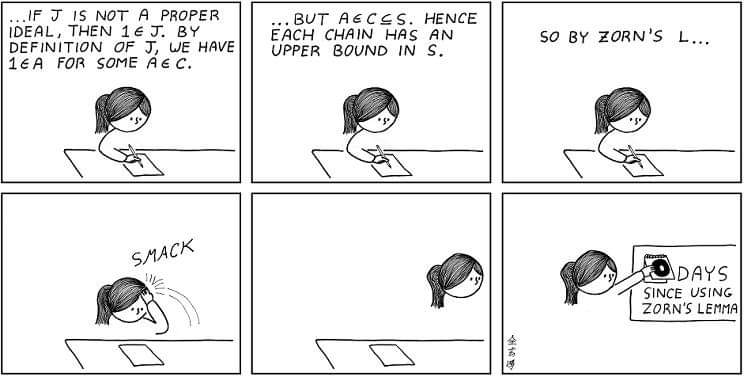
\includegraphics[width=0.75\linewidth]{figures/0DaysSinceUsingZorn.jpg}
    \caption{You reading this proof}
    \label{fig:0DyasSinceUsingZorn}
\end{figure}

Back to business: Suppose $a\notin \GL(A)$. As strongly suggested by Figure \ref{fig:0DyasSinceUsingZorn}, we shall apply the Zorn Lemma to the set $\mathscr C \coloneqq \{J \triangleleft A \mid aA \subseteq J \subsetneq A\}$ of proper ideals that contain the one generated by $a$, obtaining a maximal ideal $\mathcal J\triangleleft A$, closed by \ref{lema: ideal maximal eh fechado}.
%\vspace{-0.65cm}
\begin{quote}
    \begin{invocacao}[Zorn's Lemma]
    \label{invocacao: lema de zorn}
    If, in a non-empty and partially ordered set $\mathscr C$, every fully ordered subset has an upper quota, then $\mathscr C$ has a maximal element.
    \end{invocacao}
\end{quote}
\begin{minipage}{0.68\linewidth}
Given $x \in A \backslash \mathcal J$, notice that $\widetilde{\mathcal J} \coloneqq \{bx+j \mid b\in A, j \in \mathcal J\}$ contains properlly $\mathcal J$. Since it is maximal, $\widetilde{\mathcal J} = A$ resulting in $\sub 1A - xy \in \mathcal J$ for some $y\in A$. Hence, every non-zero element of $A/\mathcal J$ is invertible. 
\end{minipage}
\begin{minipage}{0.3\linewidth}
\begin{equation*}
\begin{tikzcd}
A \arrow[d, two heads] \arrow[rd, "\phi", dashed] &           \\
\mfrac{A}{\mathcal J} \arrow[r, "\simeq"']                  & \mathbb C
\end{tikzcd}
\end{equation*}
\end{minipage}

By Gelfand-Mazur theorem \ref{teo: Gelfand Mazur}, $A/\mathcal J \simeq \C$. Considering the canonical projection, let $\phi$ be the one who commutes the diagram at the right side. Necessarily, $\phi(\sub 1A) = 1$ and $\phi(a) = 0$ since $a\in \mathcal J$. $\hfill \square$
%\end{proof}
\vspace{0.1cm}
\begin{corolario}
\label{corol: Spec = im ev}
For a unital Banach algebra $A$, the spectrum of each element $a\in A$ coincides with the image of Gelfand transformation (\ref{eq: transformada de gelfand}), i.e.,
$\Spec a = \{\phi(a) \mid \phi \in \GGamma A\} = \Im \ev_a$.
\end{corolario}

\begin{teorema}[Gelfand-Naimark representation theorem (1943)]
\label{teo:Gelfand-Naimark}
For any commutative $C^*$-algebra $A$, Gelfand transformation (\ref{eq: transformada de gelfand}) is an isometric isomorphism between involution algebras.
\begin{proof}
Whe shall break in cases since the presence of a unity in $A$ changes compactness local to total. 
\begin{itroman}
    \item \textbf{The unital case}: By lemma \ref{lema: specm A eh localmente compacto}, ${{\GGamma}{A}}$ is a compact space and $\sub C0({{\GGamma}{A}}) = C(\GGamma A)$ is a $C^*$-algebra. By means of spectral theory, we shall prove that $\|\kappa(a)\|_\infty = \|a\|$ for all $a\in A$. For an arbitrary $\phi \in {{\GGamma}{A}}$, 
\begin{eqspaced*}{(x=x^* \in A)}
    \{\phi(x) \mid \phi \in {{\GGamma}{A}}\} \overset{\ref{corol: Spec = im ev}}= \operatorname{Spec} x \overset{\ref{lema: a*=a --> Spec a real}}\subset \R
\end{eqspaced*}
whenever $x^*=x \in A$. Therefore $\phi(x) = \con{\phi(x)}$ and hence, 
\begin{eqnarray*}
\phi(a^*) &=& \phi\Big(\dfrac{a^*+a}{2} - i\dfrac{a-a^*}{2i}\Big) \\
&=& \phi\Big(\dfrac{a^*+a}{2}\Big) - i\phi\Big(\dfrac{a-a^*}{2i}\Big) \\
&=& \con{\phi\Big(\dfrac{a^*+a}{2}\Big)} - i\,\con{\phi\Big(\dfrac{a-a^*}{2i}\Big)}\\
&=& \con{\phi\Big(\dfrac{a^*+a}{2} + i\dfrac{a-a^*}{2i}\Big)} = \con{\phi(a)}. 
\end{eqnarray*}

Since $\phi$ is arbitrary, $\kappa(a^*) = \ev_{a^*} = \con{\ev_{a}} = \con{\kappa(a)}$, thus the Gelfand transformation is an $*$-morphism. Therefore, one may notice that $\|\kappa(a)\|_\infty = \sup_{\phi \in \GGamma A} |\phi(a)| = \sup \Spec a = r(a)$ from \ref{corol: Spec = im ev}. Therefore, it follows that:
\begin{eqspaced*}{(a\in A)}
 \|\kappa(a)\|^2_\infty = \|\con{\kappa(a)} \kappa(a)\|_\infty = \|\kappa(a^*a)\|_\infty = r(a^*a) = \|a^*a\| = \|a\|^2
\end{eqspaced*}
i.e., $\kappa$ is an isometry, hence injective. Now it only rests to show that $\kappa$ is surjective.
%\vspace{-0.75cm}
 \begin{quote}
     \StoneWeierstrass
 \end{quote}
Since each isometry with Banach domain has closed image, $\Im \kappa$ is a closed dense $*$-subalgebra of $C(\GGamma A)$ containg all constant functions that separates poits, hence by Stone-Weierstra\ss\,\,\ref{teo: stone-weierstrass}, $\Im \kappa = \con{\Im \kappa} = C({{\GGamma}{A}})$, ensuring surjectivity.

\item \textbf{The non-unital case}: The proof uses the fact that both One-point compactification and unitalization constructions are pairwised: $\widetilde{\sub C0(X)} \simeq \sub C0(X \sqcup \{\infty\})$ and $\GGamma{\widetilde{A}} \simeq {{\GGamma}{A}}\sqcup \{\infty\}$. The proof comes from guaranteeing that those functors are natural transformations. Since we allready proved the ``compact-unital'' version, the ``local compact-non unital'' follows.
\end{itroman}
\end{proof}
\end{teorema}

\section{Continuos Functional Calculus}


\begin{lema}
\label{lema: usando uryshon}
Let $X\in \CHaus$ and $f \in C(X)$. If $f(\sub x{0})=0$ for some $\sub x{0} \in X$, then for every $\varepsilon>0$ there is $g \in C(X)$ such that $ \|g\|_{\infty}=1$ and $\|g f\|_{\infty}<\varepsilon$.
\end{lema}
\begin{proof}
The set $V:=\{x \in X \mid |f(x)|<\varepsilon\}$ is an open one containing $\sub{x}{0}$, because it is the pre-image of $|f(\,\cdot\,)|$ at the $\varepsilon$ ball centered at origin. Time to use some big guns from topology, in order to establish the existence of continuous extensions.
%\vspace{-0.75cm}
\begin{quote}
    \begin{invocacao}[Urysohn's Lemma - \cite{simmons1963introduction}, Theorem 28.A]
    \label{lema: urysohn}
    Let $X$ be a topological \textit{normal space}\footnote{A $T_{1}$-space (all singletons $\{x\}$ are closed) in which each pair of disjoint closed sets can be separated by open sets, in the sense that they have disjoint neighborhoods.}, and let $A$ and $B$ be disjoint closed subspaces of $X$. Then there exists a continuous real function $f$ defined on $X$, all of whose values lie in the closed unit interval $[0,1]$, such that $f(A)=0$ and $f(B)=1$.
    \end{invocacao}
\end{quote}
As stated in \cite{simmons1963introduction}, Theorem 27.A, every compact Hausdorff space is topologically normal, thus Urysohn's lemma \ref{lema: urysohn} apply: There exists $g : X \longto [0,1]$ continuous such that $g\left(\sub{x}{0}\right)=1$ and $g(x)=0$ if $ x \in V_{\neq \sub x0}$. So, $\|g\|_{\infty}=1$ and $\|g f\|_{\infty}<\varepsilon$
\end{proof}

For a unital $A \in \CstarU$, suppose that an element $a\in A$ is \textit{normal}, i.e., $a^*a=aa^*$. For each polynomial $p \in \C[z,\con z]$, we extend it to $p \in \C[a, a^*]$ in the natural way. Since $a$ is normal, $\C[a, a^*]$ is a commutative $*$-subalgebra of $A$ containing $a$ and $1$. Its closure is denoted by $C^*(1,a)$ and it is the smallest $C^*$-subalgebra of $A$ containing $1$ and $a$.

\begin{proposicao}
Let $A$ be a $C^{*}$ algebra with unity and $a \in A$ normal. 
\begin{itroman}
\item \label{prop item: GL cap C* = GL(C*)} If $b \in C^{*}(1, a)$ has an inverse $b^{-1} \in A$, then $b^{-1} \in C^{*}(1, a)$, i.e.,
\[\GL(A) \cap C^*(1,a) = \GL(C^*(1,a)).\]
\item Let $B \subset A$ be a $C^*$-subalgebra containing the unity. The same deal applies:
\begin{eqspaced*}{(1 \in B\subset A)}
\GL(A) \cap B = \GL(B).
\end{eqspaced*}
\end{itroman}
\end{proposicao}
\begin{proof}$\left.\right.$
\begin{itroman}
\item 
Suppose $b\in \GL(A)$. Since it is a commutative unital $C^{*}$-algebra, $b \notin \GL(C^*(1,a))$ if and only if $\kappa(b)$ vanishes at some point in $\GGamma{C^{*}(1, a)}$ by Gel'fand theorem \ref{teo: gelfand for BAlg com unit}. In the case which $b$ isn't invertible in the generated $C^*$-algebra, it is posssible to obtain $g \in C(\GGamma{C^{*}(1, a)})$ such that 
$$\|g\|_{\infty}=1 \e \|g\kappa(b)\|_{\infty} <\|b^{-1}\|^{-1}$$ 
by lemma \ref{lema: usando uryshon}. By the Gel'fand-Naimark representation \ref{teo:Gelfand-Naimark}, $\inv\kappa(g) \in \GGamma{C^{*}(1, a)}$ obeys $\|\inv\kappa(g)\|=\|g\|_{\infty}=1$ and
\[
\|\inv\kappa(g)b\|= \|\kappa(\inv\kappa(g) b)\|_{\infty}=\| g\kappa(b)\|_{\infty}<\|b^{-1}\|^{-1}.\] 
That inequality tells us that
$$
1=\|\inv\kappa(g)\|=\|b^{-1}(b \inv\kappa(g))\| \leq \|b^{-1}\|\|b \inv\kappa(g)\|<1,
$$
which is a contradiction. Therefore, $b \in \GL(C^*(1,a))$. $\hfill\square$

\item Notice that $\inv b = \inv{(b^*b)}b^*$ for $b \in \GL(A)$. Since $b^*b$ is a self-adjoint element, hence normal, $\inv{(b^*b)} \in C^*(1,b^*b) \subset B$ by \ref{prop item: GL cap C* = GL(C*)}. Therefore $\inv b \in B$. \qedhere
\end{itroman}
\end{proof}

\begin{corolario}[Spectral Invariance]
\label{corol: invariancia espectral}
Let $B \subset A$ be a $C^*$-subalgebra containg the unity of $A$. Therefore,
\begin{eqspaced*}{(b\in B)}
\sub \Spec B(b) = \sub \Spec A(b).
\end{eqspaced*}
\end{corolario}

\begin{contraexemplo}
Let $D \subset \C$ be the unitary open disk of complex numbers such that $|z|<1$, such that $S^1 = \partial D$. The algebra of restrictions of holomorphic functions can be given by the set:
\begin{equation*}
    E \coloneqq \{f \in C(S^1) \mid f = g\sub\restrita{S^1}, g \in C(\con D), g \sub\restrita D \in \operatorname{Hol}(D) \}
\end{equation*}
Equipped with natural complex-conjugation $f \longmapsto \con f$, $C(S^1)$ is a $C^*$-algebra, but $E$ isn't invariant by the induced involution. Therefore, the corollary \ref{corol: invariancia espectral} doesn't apply.
\end{contraexemplo}


\begin{proposicao}
\label{prop: ev_a eh homeo}
The evaluation at a normal element $a\in A$ of a unital $C^*$-algebra
\begin{equation*}
    \function{{\ev_a}{\GGamma{C^*(1,a)}}{\Spec a}{\phi}{\phi(a)}}
\end{equation*}
is a homeomorphism.
\end{proposicao}
\begin{proof}
In order to see that the image of the evaluation is in fact the spectrum, notice that $\sub\Spec{\GGamma{C^*(1,a)}}(a) = \{\ev_a(\phi) \mid \phi \in \GGamma{C^*(1,a)}\}$ by \ref{corol: Spec = im ev} and $\sub\Spec{\GGamma{C^*(1,a)}}(a) = \Spec a$ by \ref{corol: invariancia espectral}. Therefore, the evaluation is well defined and it is surjective.

Suppose that for $\phi, \psi \in \GGamma{C^*(1,a)}$, one has that $\phi(a) = \psi(a)$. Notice that for every complex polynomial $p\in \C[z,\con z]$, $\phi(p(a,a^*)) = \psi(p(a,a^*))$ since $\phi$ and $\psi$ are $*$-morphisms. The fact that $\C[a,a^*]$ is dense in $C^*(1,a)$ shows that necessarily, $\phi=\psi$, i.e., $\ev_a$ is injective.

The weak* topology is the smallest topology over $\GGamma{C^*(1,a)}$ such that each $\sub pb: \phi \longmapsto |\ev_b(\phi)|$  ($b\in C^*(1,a)$) be continuous. Therefore, for a converging net $(\phi_\alpha)_\alpha \subset \GGamma{C^*(1,a)}$, $\phi_\alpha \longto \phi$, one can see that $\ev_a$ is in fact continuous:
\begin{equation*}
    \begin{array}{rl}
     & \lim_\alpha |\ev_a(\phi_\alpha)|= \lim_\alpha p_a(\phi_\alpha)=  p_a\Big(\lim_\alpha\phi_\alpha\Big) = p_a(\phi) = |\ev_a(\phi)| \\
     \sse & \lim_\alpha \ev_a(\phi_\alpha) = \ev_a(\phi). 
\end{array}
\end{equation*}
Notice that $\GGamma{C^*(1,a)}\in \CHaus$ by lemma \ref{lema: specm A eh localmente compacto} since the inner algebra is unital. In the other direction, $\Spec a$ is compact by \ref{teo:spec eh compacto} and is Hausdorff because is a subset of the complex numbers $\C$. Since $\ev_a$ is a continuous bijection between compact Hausdorff spaces, \ref{prop: bij cont : Comp --> Haus eh homeo} guarantee us that $\ev_a$ is an homeomorphism.  
\end{proof}


\begin{teorema}[The Continous Functional Calculus]
\label{teo: calculo funcional continou}
Let $a\in A$ be a normal element of a unital $C^*$-algebra. There exists a isometric $*$-morphism $\mathfrak C_a : C(\Spec a) \longto C^*(1,a)$ such that, for every $p \in \C[a,a^*]$, with $f(z)\coloneqq p(z, \con z) = \sum_{n,m} b_{n,m}z^n {\con z}^m$, one does have
\begin{equation}
\label{eq: C(f) = f(a)}
    \mathfrak C_a(f) = \sum_{n,m} b_{n,m}a^n {(a^*)}^m = f(a).
\end{equation}
\end{teorema}
\begin{proof}
You better like composition, because this is the one! The Gel'fand transform is given by $\kappa = \ev_{(\come)} : C^*(1,a) \longto C(\GGamma{C^*(1,a)})$ and it is an $*$-isometric isomorphism (\ref{teo:Gelfand-Naimark}). By \ref{prop: ev_a eh homeo}, the composition function 
\begin{equation*}
    \function{{\ev_a^*}{C(\Spec a)}{C(\GGamma{C^*(1,a)})}{f}{f \circ \ev_a}}
\end{equation*}
also become an $*$-isometric isomorphism. Therefore the composition $\mathfrak C_a \coloneqq \inv{\kappa}\circ \ev_a^*$ holds the same title. In particular, 
\[
\mathfrak C_a(\sub1{C(\Spec {a})}) = \inv{\kappa}(\ev_a^*(\sub1{C(\Spec a)})) = \inv \kappa(\sub1{C(\Spec a)}(\ev_a)).
\]
Notice that $\sub1{C(\Spec a)} : \Spec a \longto \{1\}$. Therefore,
\begin{eqspaced*}{(\phi \in C(\GGamma{C^*(1,a)}))}
    %\hspace{-0.75cm}
    \begin{array}{rcl}
        \kappa(\mathfrak C_a(\sub1{C(\Spec {a})}))(\phi) &= & \sub1{C(\Spec a)}(\ev_a(\phi)) \\
        &=& 1 
        \\&=& \kappa(\sub 1A)(\phi).  
    \end{array}
\end{eqspaced*}
Hence $\kappa(\mathfrak C_a(\sub1{C(\Spec {a})})) = \kappa(\sub 1A)$ which imply by injectivity that $\mathfrak C_a(\sub1{C(\Spec {a})}) = \sub 1A$. One can also verify that the statement $\sub\Id{C(\Spec a)} \circ \ev_a  = \kappa(a)$, implies that $\mathfrak C_a(\sub\Id{C(\Spec a)}) = a$. Thus, (\ref{eq: C(f) = f(a)}) holds.
\end{proof}

In summary, for a normal element $a\in A$, notice $f(a) \coloneqq \kappa^{-1}(f(\ev_a))$ makes totally sense for $f\in C(\Spec a)$, extending $f: A\longto A$. Moreover, if $g \in C(f(\Spec a))$, then $g(f(a)) = (g\circ f)(a)$. Unfortunately, the continuous functional calculus does not work for non normal elements, since the generated $C^*$-algebra woudn't necessarily be commutative. 

\begin{proposicao}
Let ${A}$ and ${B}$ be two unital $C^{*}$-algebras. If $\varphi: {A} \longrightarrow {B}$ is a unital $*$-morphism, and if $a \in {A}$ is normal, then:
\begin{itroman}
\item \label{prop item: Spec varphi(a) subset Spec a}$\Spec \varphi(a) \subseteq \Spec a$,
\item if $f \in C(\Spec a)$ then $\varphi(f(a))=f(\varphi(a))$.
\end{itroman}
\end{proposicao}
\begin{proof}$\left.\right.$
\begin{itroman}
\item Suppose that $\lambda \notin \Spec a$, i.e., $\lambda 1- a\in \GL(A)$. Therefore $\lambda1-\varphi(a) = \varphi(\lambda1-a) \in \GL(B)$, hence $\lambda \notin \Spec \varphi(a)$.

\item Let $\mathscr P = \{ \ev_{(\come)}(p) : \Spec a \longto \C \mid p \in \C[z,\con z]\} \subset C(\Spec a)$. With the complex conjugation induced in those function, this is a unital $*$-subalgebra that separates points of $\Spec a$. By the Stone-Weierstra\ss\,\,(\ref{teo: stone-weierstrass}), $\mathscr P$ is dense. Therefore, there exists $(p_n)_n \subset \mathscr P$ such that $f=\lim_n p_n$. 

Since $(p_n)_n$ converges uniformly to $f$ on $\Spec \varphi(a) \subseteq \Spec a$, and by continuity of the functional calculus we conclude that:
\begin{equation*}
    \begin{array}{rcl}
        \varphi(f(a)) &=& \varphi\Big(\lim_{n\to\infty} p_n(a)\Big) \\&=& \lim_{n\to\infty} \varphi(p_n(a)) \\&=&  \lim_{n\to\infty} p_n(\varphi(a)) = f(\varphi(a)). \qedhere
    \end{array}
\end{equation*}
\end{itroman}
\end{proof}

\section{Positive elements}

\begin{definicao}
A element $a$ of a $C^*$-algebra $A$ is said to be \textit{positive} and it can be written that $a \geq 0$, whenever it is self-adjoint $a=a^*$ and its spectrum is positive: $\Spec a \subset [0,\infty)$. Hence, a order relation pops out, stating that $a\geq b$ if $a -b \geq 0$.
\end{definicao}

\begin{teorema}
\label{teo: positividade}
Let $a\in A$ be a positive element.
\begin{itroman}
\item \label{teo item: the Hahn decomposition} (The Hahn decomposition) There exists unique positive elements $a_+, a_- \in A$ such that $a = a_+-a_-$ and $a_+a_-=0$.
\item When $a$ and $-a$ are both positive, then $a= 0$.
\item \label{teo item: (lambda>=||a| : a positivo sse ||lambda-a|| =< lambda} For any $\lambda \geq \|a\|$, $a$ is positive if, and only if, $\|\lambda-a\| \leq \lambda$.
\item \label{teo item: a+b positivo} If both $a$ and $b$ are positive, so it is their sum $a+b$.
\end{itroman}
\begin{proof}$\left.\right.$
\begin{itroman}
\item Let $B \coloneqq C^*(1,a)$ be the generated unital $C^*$-algebra containing $a$, $a^*$ and $1$. By Gel'fand-Naimark theorem \ref{teo:Gelfand-Naimark}, $\kappa = \ev_{(\,\cdot\,)}$ is an isometric isomorphism between $B$ and $C(\GGamma B)$, where $\GGamma B$ is the set of non zero morphisms $\phi:B \longto \C$. Since $a$ is self-adjoint, the expansion
\begin{eqspaced*}{(\phi \in \GGamma B)}
\phi(a) = \ev_a\phi = \kappa(a)\phi = \kappa(a^*)\phi =  \phi(a^*) = \con{\phi(a)} 
\end{eqspaced*}
holds and it shows that $\kappa(a)$ must be a real continuous function. Therefore, let
\[
a_+ \coloneqq \kappa^{-1}(\max\{\kappa(a),0\}) \e a_- \coloneqq \kappa^{-1}(\min\{-\kappa(a),0\})
\]
Those elements are positive and they obey the following: $a=a_+-a_-$ and $a_+a_- = a_-a_+=0$.

\item By the Spectral Mapping theorem \ref{teo: spectral mapping}, $\Spec(-a) = -\Spec a$. Hence, both $a$ and $-a$ be positive means that $\Spec a = \{0\}$. Therefore, \ref{teo: raio espectral} guarantee us that $\|a\|=r(a)=0$, i.e., $a=0$.

\item Let $\lambda \geqslant \|a\|$. Notice that by \ref{lema:lambda1-a invertivel para ||a||<lambda} and \ref{lema: a*=a --> Spec a real}, $\Spec a \subset [-\|a\|,\|a\|] \subset [-\lambda,\lambda]$. Therefore,
\[
\|\lambda-a\| = r(\lambda-a) = \sup \Spec(\lambda-a)  = \sup_{\mu \in \Spec a} |\lambda-\mu| 
\]
Hence $\|\lambda-a\| \leqslant \lambda$ if and only if $\Spec a \subset [0,\infty)$.
\item By \ref{teo item: (lambda>=||a| : a positivo sse ||lambda-a|| =< lambda}, $\|\|x\|-x\| \leq \|x\|$ for $x\in \{a,b\}$. Therefore:
\begin{equation*}
\big\|\|a\|+\|b\|-\|a+b\|\big\| \leq \|\|a\|-a\|+\|\|b\|-b\| \leq \|a\|+\|b\|
\end{equation*}
So \ref{teo item: (lambda>=||a| : a positivo sse ||lambda-a|| =< lambda} again ensures that $a+b$ is positive.
\end{itroman}
\end{proof}
\end{teorema}


A \textit{square root} of an element $a\in A$ is a element $b\in A$ such that $b^2=a$.

\begin{teorema}
\label{teo: a raiz quadrada}
Each positive element $a\geqslant 0$ of a $C^*$-algebra $A$ has a unique positive square root.
\begin{proof}
Since positive elements are normal, we are good to go. Pick the usual square root $\sqrt{\come}$ defined on the interval $[0, \|a\|] \supset \Spec a$. With the continuous functional calculus \ref{teo: calculo funcional continou}, notice that $\sqrt{a} \coloneqq \mathfrak C_a(\sqrt{\come}) = \inv\kappa(\sqrt{\ev_a})$ is a well defined element of $A$, self-adjoint since and the square root $\sqrt{\come}$ is a real-valued function. Moreover, $\Spec \sqrt a = \sqrt{\Spec a} \subset [0,\infty)$, i.e., $\sqrt{a} \geq 0$. 

The notation wasn't choose randomly: For $p(x) \coloneqq x^2$, notice that $p \in C(\sqrt{\Spec a})$, hence $\sqrt{a}^2 = p(\sqrt{a}) = (p \circ \sqrt{\come})(a) = a$. If $\sub b1, \sub b2$ were two positives square roots of $a$, $\sub b1^2 = a = \sub b2^2$, one can see that $\sub b1 = \sqrt{\sub b1^2} = \sqrt{a}  = \sqrt{\sub b2^2} = \sub b2$, concluding uniqueness.
\end{proof}
\end{teorema}


%\begin{invocacao}[\cite{ogasawara1955theorem}]
%Let $A$ be a $C^*$-algebra. Then for every $a,b \in A^u$:
%\begin{itroman}
%\item If $a\geqslant b$, then $\sqrt a \geqslant \sqrt b$.
%\item If $0\leq a \leq b$ implies allways $a^2 \geqslant b^2$, then $A$ is commutative.
%\end{itroman}
%\end{invocacao}

\begin{lema}
\label{lema: a positive sse a=b(star)b}
Let $A$ be a unital $C^*$-algebra and $a\in A$. The following are equivalent:
\begin{itroman}
\item $a$ is positive.
\item There is a self-adjoint element $b \in A$ such that $b^{2}=a$.
\item There is $b \in A$ such that $b^{*} b=a$.
\end{itroman}
\end{lema}
\begin{proof}
The implication $(i) \Rightarrow (ii)$ is essentialy the theorem \ref{teo: a raiz quadrada} and $(ii) \Rightarrow (iii)$ is trivial. 
\begin{itemize}
    \item[$(iii) \Rightarrow (i)$] If $a= b^*b$, let $a_+$ and $a_-$ be the Hahn decomposition such as in \ref{teo: positividade}\ref{teo item: the Hahn decomposition}. Notice that
    \[-(ba_-)^* (ba_-) = -a_- b^*ba_- = -a_-(a_+-a_-)a_- = (a_-)^3\]
    Since it is a positive element, $\Spec a^3 = (\Spec a)^3$ \textcolor{red}{CONTINUAR} \qedhere
\end{itemize}
\end{proof}


\begin{lema}
\label{lema:a<b --> b^-1 < a^-1}
Whenever $0 \leq a \leq b$ are invertible elements in a unitary $C^*$-algebra $A$, then $\inv b \leq \inv a$.
\end{lema}
\begin{proof}
Given two self-adjoint elements $x,y \in A$ such that $x\leq y$, notice that $z^*xz \leq z^*yz$ for all $z$. Indeed, since $x-y \geq 0$, 
\begin{eqspaced*}{(z\in A)}
\begin{array}{rcl}
    z^*yz - z^*xz &=& z^*(x-y)z \\
    &=& z^*(\sqrt{x-y})^*(\sqrt{x-y}) z \\
    &=& (\sqrt{x-y}\,z)^*(\sqrt{x-y}\,z) \overset{\ref{lema: a positive sse a=b(star)b}}\geq 0\\
    & & \\
    \To z^*xz &\leq & z^*yz
\end{array}
\end{eqspaced*}
Since $b-a\geq 0$, the above shows that
\begin{equation*}
    \begin{array}{rcl}
        0 &\leq& \inv{\sqrt b}\,(b-a)\,\inv{\sqrt b} \\
        &=& \inv{\sqrt b}\,{b}\,\inv{\sqrt b} - \inv{\sqrt b}\,a\,\inv{\sqrt b} \\
        &=& 1- \inv{\sqrt b}a\inv{\sqrt b}
    \end{array}
\end{equation*}
Thus, $(\sqrt{\vphantom{b}a} \sqrt{b}^{-1})^{*}(\sqrt{\vphantom{b}a} \sqrt{b}^{-1}) \leq 1$, implying that $\| \sqrt{\vphantom{b}a} \sqrt{b}-1 \| \leq 1$. Hence,
\[{1} \geq (\sqrt{\vphantom{b}a} \sqrt{b}^{-1})(\sqrt{\vphantom{b}a} {\sqrt{b}}^{-1})^{*}=\sqrt{\vphantom{b}a} b^{-1} \sqrt{\vphantom{b}a}\]
Multiplying on both sides by $\sqrt{\vphantom{b}a}^{-1}$, we get
$$
a^{-1}=\sqrt{\vphantom{b}a}^{-1}\, 1\, \sqrt{\vphantom{b}a}^{-1} \geq \sqrt{\vphantom{b}a}^{-1} \,(\sqrt{\vphantom{b}a} \, b^{-1} \sqrt{\vphantom{b}a})\, \sqrt{\vphantom{b}a}^{-1}=b^{-1}.
$$
\end{proof}

\begin{lema}
\label{lema:||a||=inf(lambda | a <= lambda)}
If $a\in A$ is a positive element of a unital $C^*$-algebra, then 
\begin{equation*}
    \|a\|=\inf\{\lambda \geqslant 0 \mid a \leqslant \lambda \cdot 1\}.
\end{equation*}
\end{lema}
\begin{proof}
Notice that $\|a\| \in \{\lambda \geqslant 0 \mid a \leqslant \lambda \cdot 1\}$, because the function $t \longmapsto t-\|a\|$ is positive: Since $\|a\|\leqslant \|a\|$,  $\|a\|1-a$ isn't invertible by \ref{lema:lambda1-a invertivel para ||a||<lambda}, hence $\|a\|\in \Spec a$.
\end{proof}

\begin{corolario}
\label{lema: Cstar prop: a <= b ---> |a| <= |b|}
Let $A$ be a $C^*$-algebra and $a,b\in A$. Therefore $0\leqslant a \leqslant b \Rightarrow \|a\|\leqslant \|b\|$.
\end{corolario}

\section{Approximate Units}
We can always trade unitary arguments with approximate units over Banach algebras, which is exactly what are we going to do. Traditionally in topology, nets can be much more useful to describe weird continuous functions spaces than sequences are, and, as long as Banach, $C^*$ and Von-Neumann algebras are blazingly wild, we need to appeal to these objects.

%We can allways embed $A$ into their unifization $A^u \simeq A \oplus \C$, such that $A$ can be seen as a ideal in which $A^u/A \simeq \C$.

\begin{definicao}[Approximate Unit]
Let $(\LLambda, \preceq)$ be an pre-ordered set\footnote{For $\lambda, \lambda'\in \LLambda$, there exists a $\mu$ which both $\lambda \preceq \mu$ and $\lambda'\preceq \mu $. Equivalently, any finite subset has an upper bound.}. The image of any function $\LLambda \longto A$ will be said to be a \textit{net}, and will be mentioned as $(\sub{u}{\lambda})_{\lambda \in \LLambda}$. An \textit{approximate unit net} will allways denote a net $(\sub{u}{\lambda})_{\lambda \in \LLambda}$ such that $0 \leq \Anorm{\sub{u}{\lambda}} \leq 1$  and
\begin{eqspaced*}{(a\in A)}
\lim_{\lambda\in \LLambda}\|a-a\sub{u}{\lambda}\|  = 0 \hphantom{=}\Big(= 
\lim_{\lambda\in \LLambda}\|a-\sub{u}{\lambda} a\|\Big)
\end{eqspaced*}
which means that: for every $\ep>0$, exists $\sub \lambda0 \in \LLambda$ such that $\|a-a\sub{u}{\lambda}\| < \ep$ whenever $\lambda \succeq \sub\lambda0$. Therefore, we can stabilish that $\lim_\lambda a\sub u\lambda = \lim_\lambda \sub u\lambda a = a$ for every element $a$.
\end{definicao}

Notice that for any complex $z$, $\delta \in [0,1)$ can allways be chosen such that $|z-z\delta|$ is desirily small (with respect to the ordinarily euclidean norm), i.e., the non-negative numbers with norm less than one $[0,1) = (\delta)_{\delta \in [0,1)}$ is a approximate unit over the complex numbers. We'll show that those in fact exists in each and every $C^*$-algebra.

\begin{teorema}
The positive elements of any $C^*$-algebra $A$ with norm less than one are a approximate unit.
\end{teorema}
\begin{proof}
Let $\LLambda \coloneqq \{a\in A \mid a \geq 0 \text{ and } \|a\| < 1\}$. To show that $\LLambda$ is directed set, we invoque functional calculus by our side:  
\begin{itroman}
\item \textbf{$\boldsymbol{\LLambda}$ is a pre-ordered set}: Consider the bijection:
%\begin{minipage}{0.35\linewidth}
\begin{equation*}
    \functionwithinverse{g{[0,1)}{[0,\infty)}{t}{\dfrac{t}{1-t}}t{1-\dfrac{1}{1+t}}}
\end{equation*}
%\end{minipage}
%\hfill
%\begin{minipage}{0.55\linewidth}
%\begin{figure}[H]
%    \centering
%    \begin{tikzpicture}[scale=2, xscale = 2]
%    \draw[->] (-0.05, 0) -- (0.55, 0) node[right] {$x$};
%  \draw[->] (0, -0.05) -- (0, 1.05) node[above] {$y$};
%  \draw[domain=0:0.5, smooth, variable=\x, blue] plot ({\x}, {\x/(1-\x)}) node[right] {$g$};
%  \draw[domain=0:0.5, smooth, variable=\x, red] plot ({\x}, {1-1/(1+\x)}) node[right] {$g^{-1}$};
%    \end{tikzpicture}
%    \caption{Graph of $g$ and $\inv g$}
%\end{figure}
%\end{minipage}
Since $g$ and $g^{-1}$ map $0$ to $0$, they will send $A$ to $A$ under the functional calculus, even if $A$ is non-unital. Use the order $\geq$ in $\LLambda$ induced by the positive elements in $A$. Now choose $a, a'\in \LLambda$ and define:
$$b \coloneqq g^{-1}(g(a)+g(a'))=1-(1+g(a)+g(a'))^{-1}.$$
Then $\Spec b \subset [0,1)$ so $b\in \LLambda$. Also, since $1+g(a)+g(a') \geq 1+g(a)$, lemma \ref{lema:a<b --> b^-1 < a^-1} implies that
$$
b=1-(1+g(a)+g(a'))^{-1} \geq 1-(1-g(a))^{-1}=g^{-1}(g(a))=a.
$$
Likewise $b \geq a'$. 
\item \textcolor{red}{CONTINUAR}
\qedhere
\end{itroman}
\end{proof}

